%Napisać gdzie używa się tego algorytmu
%Opisać sposób działania programu/algorytmu
%Napisać spsoób wykorzystania algorytmu po przez wykonanie przykładu (np. mnożenie macierzy - wykonać ręcznie przykład z mnożeniem macierzy pokazujący jak mnoży się macierz ręcznie)
%Jeśli zadanie zakłada przedstawienie jakiegoś narzędzia (np. git, AI) należy opisać narzędzie

\newpage
\section{Analiza problemu}

Drzewa wyszukiwań binarnych (BST - Binary Search Trees) są strukturami danych szeroko stosowanymi w informatyce ze względu na ich efektywność w przechowywaniu danych i szybkim dostępie do nich. Celem tego rozdziału jest analiza kontekstu, w którym algorytm BST znajduje zastosowanie, omówienie jego działania oraz przedstawienie praktycznego przykładu implementacji i użytkowania. Wygląd przykłądowego dzrzewa BST widać na rysunku \textbf{2.1}\footnote{Zdjęcie ze strony  \url{https://en.wikipedia.org/wiki/Binary_search_tree/}\cite{www2}}

\begin{figure}[htb!]
	\centering
	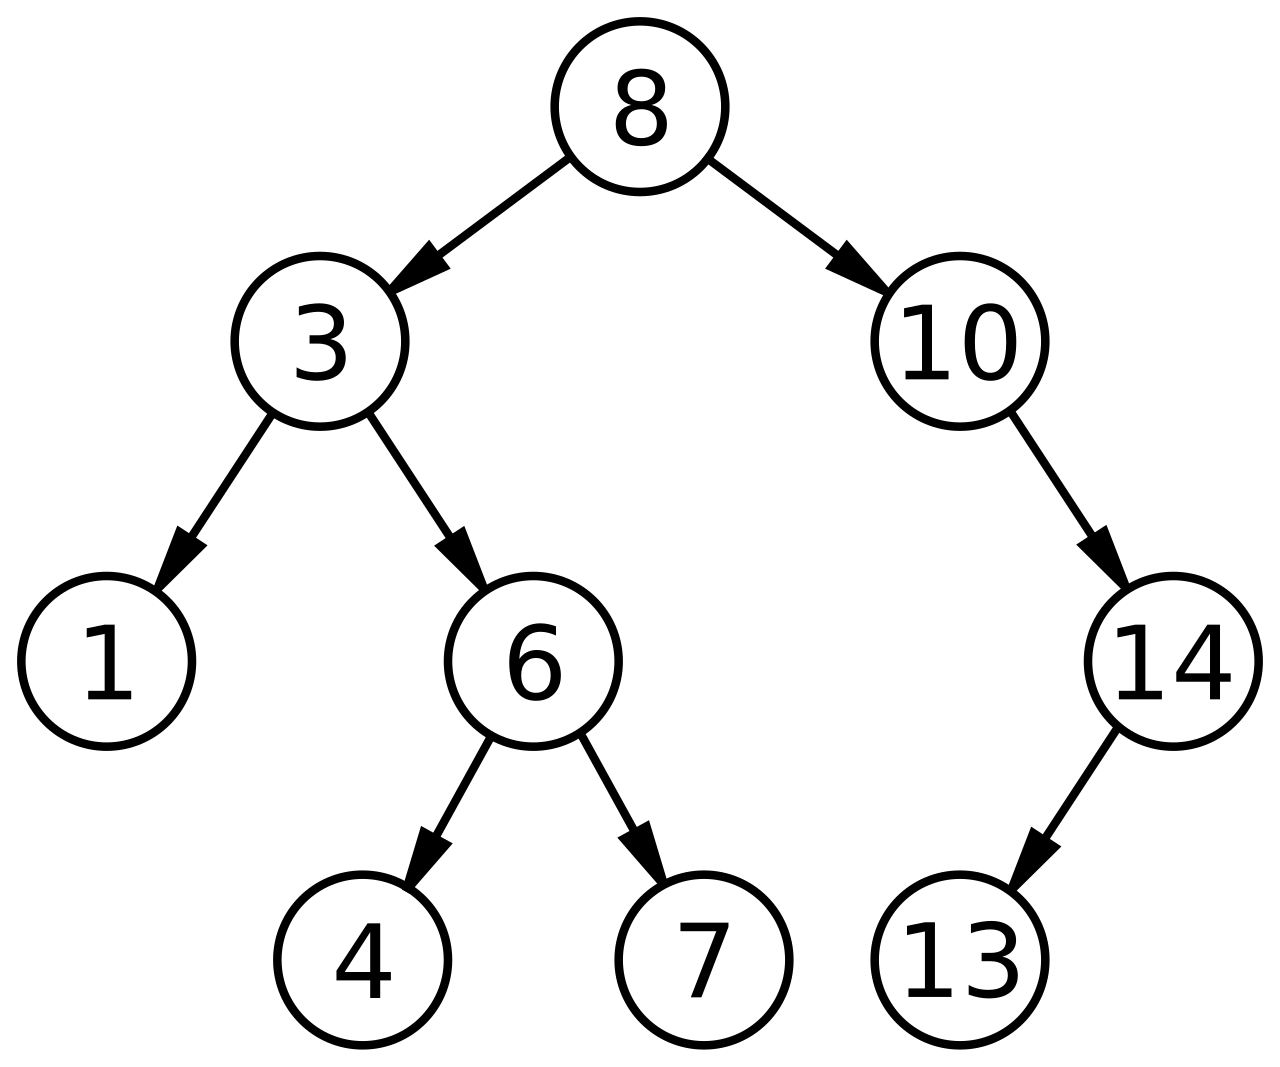
\includegraphics[width=0.8\linewidth]{rys/bst.png}
	\caption{Przykładowy wygląd BST}
\end{figure}

\subsection{Zastosowanie algorytmu BST}

Drzewo wyszukiwań binarnych jest używane wszędzie tam, gdzie konieczne jest szybkie przechowywanie i przetwarzanie danych uporządkowanych. Przykłady zastosowań BST obejmują:
\begin{itemize}
	\item \textbf{Bazy danych:} BST są często używane w strukturach danych baz danych, gdzie kluczowe jest szybkie wyszukiwanie rekordów.
	\item \textbf{Systemy plików:} W systemach plików drzewa wyszukiwań mogą służyć do organizacji katalogów, ułatwiając wyszukiwanie i zarządzanie plikami.
	\item \textbf{Słowniki i systemy słów kluczowych:} W aplikacjach, które operują na dużych zbiorach słów, takich jak słowniki czy autokorekta, BST zapewniają szybki dostęp do danych.
	\item \textbf{Struktury indeksowe:} BST są podstawą wielu struktur indeksowych wykorzystywanych w algorytmach i systemach, które potrzebują sortowanego dostępu do danych.
\end{itemize}

\subsection{Sposób działania algorytmu}

Algorytm drzewa BST jest oparty na zasadzie rekurencyjnej struktury, gdzie każdy węzeł drzewa przechowuje element z kluczem oraz dwa wskaźniki - lewy i prawy. Struktura BST zapewnia, że dla każdego węzła wszystkie klucze w lewym poddrzewie są mniejsze od klucza w węźle, a wszystkie klucze w prawym poddrzewie są większe. Dzięki tej strukturze BST umożliwia szybkie przeszukiwanie drzewa.

Podstawowe operacje na drzewie BST to:
\begin{itemize}
	\item \textbf{Dodawanie elementu:} Przeszukując drzewo od korzenia, porównujemy wartość klucza nowego elementu z wartościami istniejących węzłów, aż znajdziemy odpowiednie miejsce do jego dodania jako liść drzewa.
	\item \textbf{Przeszukiwanie drzewa:} Przechodzimy po węzłach drzewa, porównując wartości w celu znalezienia ścieżki do określonego elementu.
	\item \textbf{Wyświetlanie drzewa:} Istnieją różne sposoby wyświetlania drzewa, takie jak preorder, inorder, i postorder, które odwiedzają węzły w określonej kolejności.
\end{itemize}

\subsection{Przykład działania algorytmu BST}

Poniżej znajduje się przykładowa operacja dodawania elementów do drzewa BST. Załóżmy, że mamy pustą strukturę i chcemy dodać elementy w kolejności: 15, 10, 20, 8, 12.

\begin{enumerate}
	\item Dodajemy element \textbf{15} jako korzeń drzewa, ponieważ jest to pierwszy element.
	\item Element \textbf{10} jest mniejszy niż 15, więc staje się lewym potomkiem korzenia.
	\item Element \textbf{20} jest większy niż 15, dlatego staje się prawym potomkiem korzenia.
	\item Element \textbf{8} jest mniejszy niż 15 oraz mniejszy niż 10, więc zostaje lewym potomkiem węzła o wartości 10.
	\item Element \textbf{12} jest mniejszy niż 15, ale większy niż 10, więc zostaje prawym potomkiem węzła o wartości 10.
\end{enumerate}

Po dodaniu tych elementów, BST przyjmuje następującą formę (Rysunek \textbf{2.2}\footnote{Zdjęcie ze strony  \url{https://treeconverter.com/?input=15,10,20,8,12}\cite{www3}}):

\begin{figure}[htb!]
	\centering
	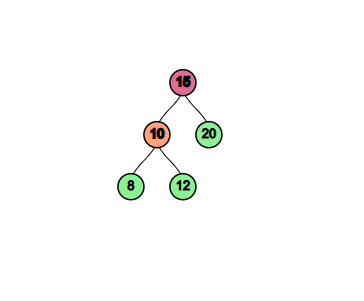
\includegraphics[width=0.7\linewidth]{rys/bstvisul.png}
	\caption{Zilustrowane BST z danymi}
\end{figure}

\subsection{Git - narzędzie do kontroli wersji}

Git jest narzędziem umożliwiającym zarządzanie wersjami kodu źródłowego w zespołach programistycznych, co jest kluczowe dla poprawnego zarządzania projektem, szczególnie przy współpracy zespołowej. W projekcie tym, Git pozwala na:
\begin{itemize}
	\item \textbf{Równoległą pracę na gałęziach:} Każdy członek zespołu może pracować niezależnie na swojej gałęzi, a po zakończeniu pracy zmiany są scalane do gałęzi głównej.
	\item \textbf{Śledzenie historii commitów:} Każda zmiana w kodzie jest zapisywana w historii, co pozwala na łatwe cofanie zmian lub śledzenie poprawek.
	\item \textbf{Rozwiązywanie konfliktów:} Git umożliwia kontrolę nad sytuacjami, gdy zmiany w kodzie kolidują, pozwalając użytkownikom na ręczne rozwiązywanie konfliktów i sprawdzanie ich.
\end{itemize}

W kolejnym rozdziale omówimy szczegóły implementacyjne, takie jak struktura klas i operacje realizowane przez algorytm BST w naszej aplikacji.
